\documentclass[twoside]{article}

\usepackage{aistats2020}
% If your paper is accepted, change the options for the package
% aistats2020 as follows:
%
%\usepackage[accepted]{aistats2020}
%
% This option will print headings for the title of your paper and
% headings for the authors names, plus a copyright note at the end of
% the first column of the first page.

% If you set papersize explicitly, activate the following three lines:
%\special{papersize = 8.5in, 11in}
%\setlength{\pdfpageheight}{11in}
%\setlength{\pdfpagewidth}{8.5in}

% If you use natbib package, activate the following three lines:
\usepackage[round]{natbib}
\renewcommand{\bibname}{References}
\renewcommand{\bibsection}{\subsubsection*{\bibname}}

% If you use BibTeX in apalike style, activate the following line:
\bibliographystyle{apalike}

% graphics
\usepackage{float}
\usepackage{graphicx}

% math and stuff
\usepackage{amssymb}
\usepackage{amsmath}
\usepackage{amsthm}
\usepackage{algorithm}
\usepackage{algorithmicx}
\usepackage{algpseudocode}
%\newcommand{\disc}{\mathrm{disc}}
%\newcommand{\cont}{\mathrm{cont}}
%\newcommand{\tr}{\mathtt{tr}}
%\newcommand{\model}{\mathcal{P}}
%\newcommand{\proposal}{\mathcal{Q}}
\newtheorem{theorem}{Theorem}[section]
\newtheorem{corollary}{Corollary}[theorem]
\newtheorem{lemma}[theorem]{Lemma}

\begin{document}

% If your paper is accepted and the title of your paper is very long,
% the style will print as headings an error message. Use the following
% command to supply a shorter title of your paper so that it can be
% used as headings.
%
%\runningtitle{I use this title instead because the last one was very long}

% If your paper is accepted and the number of authors is large, the
% style will print as headings an error message. Use the following
% command to supply a shorter version of the authors names so that
% they can be used as headings (for example, use only the surnames)
%
%\runningauthor{Surname 1, Surname 2, Surname 3, ...., Surname n}

\twocolumn[

\aistatstitle{Automated Involutive MCMC}

\aistatsauthor{ Marco Cusumano-Towner \And Alexander K. Lew \And Vikash K. Mansinghka }

\aistatsaddress{ Massachusetts Institute of Technology } ]

\begin{abstract}
Involutive MCMC is a unifying framework for MCMC that encompasses many standard
and recent MCMC algorithms from the literature, from reversible jump MCMC to
Hamiltonian Monte Carlo to kernels based on deep neural networks. The key idea
in involutive MCMC is that a combination of (i) an auxiliary probability
distribution and (ii) an involution on the extended state space that includes
the model latent variables and the auxiliary variables results in MCMC kernels
that satisfy detailed balance with respect to the target distribution. The
involutive MCMC framework is appealing for its simplicity and generality, and
promises to be a useful conceptual and mathematical tool for exploring the
design space of MCMC kernels. However, like other Monte Carlo samplers,
implementing involutive samplers is time consuming and error prone. This paper
describes a technique for automatically generating the implementation of
involutive MCMC samplers from two probabilistic programs that define the target
distribution and the auxiliary probability distribution respectively, and a
differentiable program that defines the involution. The technique also detects
common conceptual and programming errors that arise when designing and
specifying involutive MCMC algorithms. This paper describes the support for
involutive MCMC in the Gen probabilistic system that uses this technique, and
shows involutive samplers specified using Gen's high-level probabilistic and
differentiable programming languages.
\end{abstract}

\section{INTRODUCTION}

%This is the best paper~\citep{cusumano2019gen}.

\subsection{Second Level Heading}

\subsubsection{Third Level Heading}

\paragraph{Fourth Level Heading}

\section{BACKGROUND AND RELATED WORK}

%\subsection{Traces}

\begin{figure*}[ht]
    \centering
    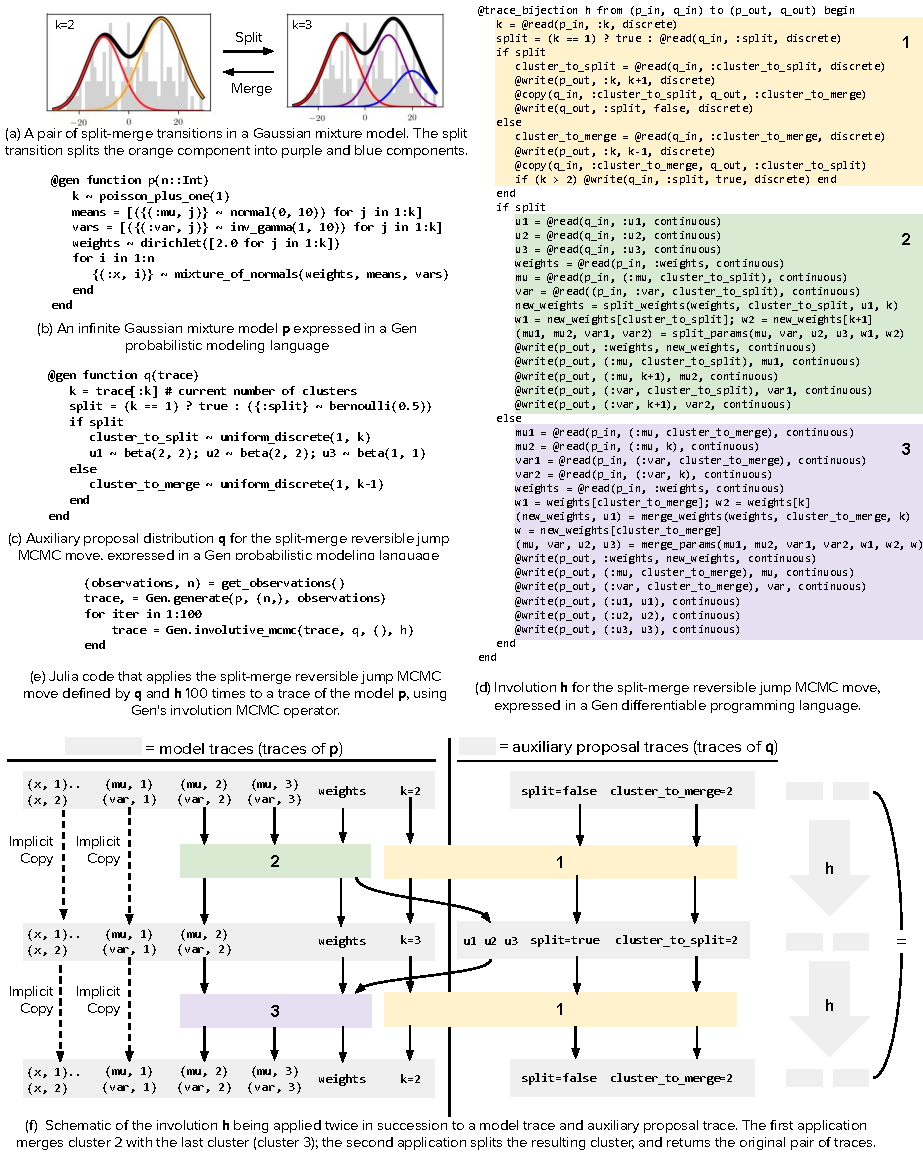
\includegraphics[width=\textwidth]{figures/mixture.pdf}
    \caption{
Example of reversible jump MCMC~\citep{green1995reversible} implemented using involutive MCMC in Gen.
The example implements a `split-merge move' in a infinite Gaussian mixture model~\citep{richardson1997bayesian} using three Gen programs:
(1) a probabilistic program $\mathtt{p}$ encoding the generative model (shown in b),
(2) a probabilistic program $\mathtt{q}$ encoding an auxiliary probability distribution (shown in c),
and (3) a differentiable program $\mathtt{h}$ that encodes an involution on the space of pairs of traces of $\mathtt{p}$ and $\mathtt{q}$ (shown in d).
Gen's involutive MCMC operator (shown in e) automatically computes the acceptance probability.
}
    \label{fig:mixture}
\end{figure*}

\begin{figure*}[ht]
    \centering
    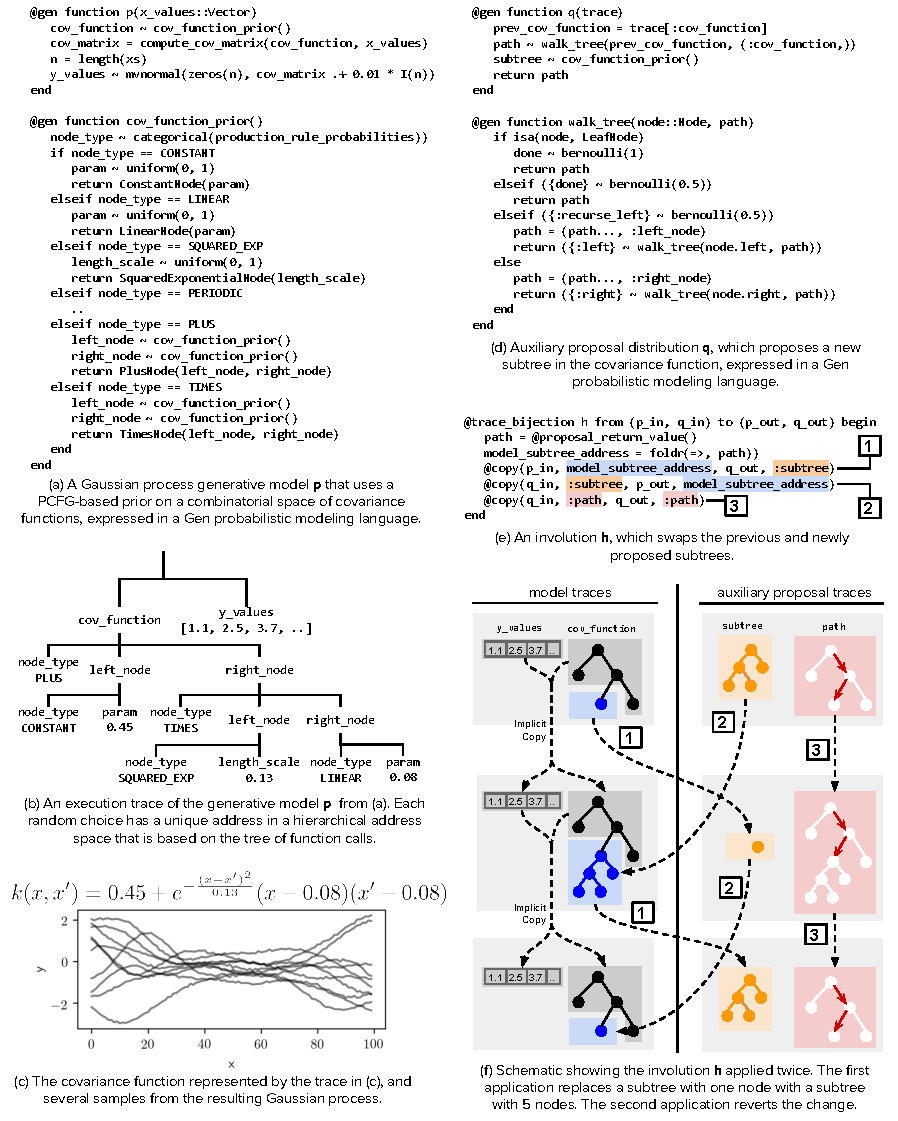
\includegraphics[width=\textwidth]{figures/structure-learning.pdf}
    \caption{
A mixture kernel implemented using involutive MCMC in Gen, applied to infer the covariance function of a Gaussian process.
The prior on covariance functions is based on a probabilistic context-free grammar.
Each component kernel in the mixture replaces a subtree of the covariance function parse tree with a new subtree.
The mixture kernel chooses a random subtree to replace via a random walk on the parse tree.
The mixture kernel is composed from three Gen programs:
(1) a probabilistic program $\mathtt{p}$ encoding the generative model (shown in a),
(2) a probabilistic program $\mathtt{q}$ encoding an auxiliary probability distribution (shown in b), and
(3) a differentiable program $\mathtt{h}$ that encodes an involution (shown in d).
}
    \label{fig:structure-learning}
\end{figure*}

\section{INVOLUTIVE MCMC}
Let $p$ denote the target probability density with respect to some $\sigma$-finite measure $\mu_X$ on a set $X$.
For each $x$ such that $p(x) > 0$, let $q_x$ denote a probability density with respect to some $\sigma$-finite measure $\mu_U$ on a set $U$.
Let $\mu := \mu_X \times \mu_U$ denote the product measure on the space $X \times U$, and let $\pi(x, u) := p(x) q_x(u)$ and $Z := \{(x, u) : \pi(x, u) > 0\}$.
Let $f : Z \to Z$ denote an involution ($f^{-1} = f$) such that the pushforward of $\mu$ under $f$, denoted $\mu \circ f^{-1}$, is absolutely continuous with respect to $\mu$, with Radon-Nikodym derivative $d (\mu \circ f^{-1}) / d\mu : Z \to [0, \infty)$.

\begin{algorithm}[h]
\begin{algorithmic}
\Procedure{involutive-mcmc-move}{$p$, $q$, $f$, $x$}
    \State $u \sim q(\cdot; x)$ \Comment{Sample auxiliary variables}
    \State $(x', u') \gets f(x, u)$ \Comment{Apply involution}
    %\State $\alpha \gets
        %\frac{p(x') q(u'; x')}{p(x) q(u; x)} \left| \left[ \frac{\partial h(u, t)}{\partial (u, t)} \right] \right|$
    % TODO or should we show the Radon-Nikodym derivative?
    \State $\alpha \gets
        \displaystyle \frac{p(x') q_{x'}(u')}{p(x) q_{x}(u)} \left( \frac{d (\mu \circ f^{-1})}{d \mu} (x, u)\right)$
    % TODO check it
    \State $r \sim \mathrm{Uniform}(0, 1)$
    \State \algorithmicif \, $r \le \alpha$ \algorithmicthen \, \Return $x'$ \algorithmicelse \, \Return $x$ 
\EndProcedure
\end{algorithmic}
\caption{Involutive MCMC}
\label{alg:involutive-mcmc}
\end{algorithm}
See Section~\ref{sec:radon-nikodym-special-case} for a derivation of the Radon-Nikodym derivative $d (\mu \circ f^{-1}) / d \mu$ for a special case, when the involution $f$ can be factored into (i) an involution on a countable partition of $Z$ and (ii) a family of continuously differentiable bijection on Euclidean spaces.

\begin{theorem}[Involutive MCMC is stationary]
For $p$, $q$, and $f$ satisfying the requirements above, Algorithm~\ref{alg:involutive-mcmc} defines a probability kernel on $X$ that is stationary with respect to the distribution $p$.
\end{theorem}
\begin{proof}
The proof is presented in stages in the appendix (see Section~\ref{sec:involution-detailed-balance}, Section~\ref{sec:involution-is-stationary}, and Section~\ref{sec:involutive-mcmc-is-stationary}).
\end{proof}

%\begin{lemma}\label{lemma:involution-detailed-balance} % TODO cite
%For $p$, $q$, and $f$ satisfying the properties above, let $k'$ denote the following transition kernel on $Z$:
%\[
%k'_z(A) := [f(z) \in A] \alpha(z) + [z \in A](1 - \alpha(z))
%\]
%The transition kernel $k'$ on $Z$ defined by the involution $f$ satisfies detailed balance with respect to $\pi$:
%\[
%\int_B k'_z(A) \pi(dz) = \int_A k'_z(B) \pi(dz) \mbox{ for all } A, B \in \Sigma_Z
%\]
%And in particular it is stationary with respect to $\pi$:
%\[
%\int_Z k'_z(A) \pi(dz) = \pi(A) \mbox{ for all } A \in \Sigma_Z
%\]
%\end{lemma}
%\begin{proof}
%\end{proof}
%
%\begin{theorem}\label{theorem:stationarity}
%The transition kernel $k$ on $X$ defined by Algorithm~\ref{alg:involutive-mcmc} for valid $p$, $q$, and $f$:
%\[
%k_x(A) := \int_U k'_{x,u}(A \times U) q_x(u) \mu_U(du) \;\; \mbox{for all} \;\; A \in \Sigma_X, x \in X
%\]
%is stationary with respect to $p$.
%\end{theorem}
%\begin{proof}
%By Lemma~\citep{lemma:involution-detailed-balance}, the transition kernel $k'$ is stationary with respect to $\pi$:
%\[
%%\int_B k'_{z}(B) \pi(z) \mu(dz) = \pi(B) \mbox{ for all } z \in X \times U, B \in \Sigma_Z
%\]
%It suffices to show that
%\begin{align*}
%\int_X k_x(A) p(x) \mu_X(dx) &= p(A) \mbox{ for all } A \in \Sigma_X\\
%\int_X \left( \int_U k'_{x,u}(A \times U) q_x(u) \mu_U(du) \right) p(x) \mu_X(dx) &= p(A)\\
%\int_{X \times U} k'_{x,u}(A \times U) q_x(u) p(x) \mu(dz) &= p(A)
%\end{align*}
%By Lemma~\citep{lemma:involution-detailed-balance}, setting $B := X \times U$, the left-hand-side is:
%\[
%\pi(X \times U) = \int_X \int_U p(x) q_x(u) \mu(
%\]
%\end{proof}
%\paragraph{Detailed balance of the involution}
%%Let $q_
%
%\paragraph{Stationarity}
%
%\paragraph{Conditional distribution and observations fixed}

% TODO PyTorch implementation??

\section{AUTOMATIC ACCEPTANCE PROBABILITY CALCULATION}

\subsection{Exploiting Jacobian Sparsity}

% TODO can only show this for a special case -- discrete involution + continuous?, or some more general case?

% TODO show an performance table of moves per second with and without the sparsity reduction (?)

\section{A DYNAMIC CHECK FOR DETECTING BUGS}

% TODO show an example of the type of bug it can detect (an edge case?)

\section{EXAMPLES}


\subsubsection*{Acknowledgements}
All acknowledgments go at the end of the paper, including thanks to reviewers who gave useful comments, to colleagues who contributed to the ideas, and to funding agencies and corporate sponsors that provided financial support.

\bibliography{references} 

\clearpage
\onecolumn
\section*{APPENDIX}

%\subsection{Distributions on traces}
%% TODO rewrite this section..
%Define target density $\pi$ (XXX below it is called $p$, fix this) on the joint space $X \times U$, where $X$ are traces of the model and $X$ are traces of the proposal, in terms of the density $p(x)$ and the family of densities $q_x(u)$ as $\pi(x, u) := p(x) q_u(x)$.
%
%% TODO rename the joint target density to \pi below
%We want to show stationarity with respect to $\pi$, using stationarity of the involution with respect to the joint density (below).
%\begin{equation}
%\int_X p(x) \ell_x(A) \mu(dx) = p(A) \mbox{ for all } A \in \Sigma
%\end{equation}
%where $\ell_x(A)$ is the probability of transitioning into set $A$ from $x$, and is given by:
%\begin{equation}
%\ell_x(A) := \int_U k_{(x, u)}(A \times U) \mu(du)
%\end{equation}
%where $k_{(x, u)}$ is the measure on $X \times U$ that is induced by applying the involution $h$ to the state $(x, u)$.
% TODO checkme


\subsection{Derivation of the pushforward Radon-Nikodym derivative for a special case} \label{sec:radon-nikodym-special-case}
Implementing Algorithm~\ref{alg:involutive-mcmc} requires computing the Radon-Nikodym derivative $d (\mu \circ f^{-1}) / d \mu$.
This section derives that function for the special case in which the involution $f$ can be factored into an involution on a countable set $I$ and a family of bijections on $\mathbb{R}^{n_i}$ for some $n_i$ for each $i \in I$.
Suppose $Z = \{(i, \mathbf{x}) : i \in I, \mathbf{x} \in \mathbb{R}^{n_i}\}$.
Suppose $f_1$ is an involution on $I$ and $n_i = n_{f_1(i)}$ and $f_2$ is a family of continuously differentiable bijections indexed by $i \in I$, such that $f_{2,i} : \mathbb{R}^{n_i} \to \mathbb{R}^{n_i}$.
Also suppose that $f_{2,i} = f_{2,f_1(i)}^{-1}$ for all $i \in I$. That is,
\begin{equation}
f_{2,i}(f_{2,f_1(i)}(\mathbf{x})) = \mathbf{x} \mbox{ for all } \mathbf{x} \in \mathbb{R}^{n_i} \mbox{ and all } i \in I
\end{equation} 
Then, $f : Z \to Z : (i, \mathbf{x}) \mapsto (f_1(i), f_{2,i}(\mathbf{x}))$ is an involution because:
\begin{equation}
f(f(i, \mathbf{x})) = f(f_1(i), f_{2,i}(\mathbf{x})) = (f_1(f_1(i)), f_{2,f_1(i)}(f_{2,i}(\mathbf{x}))) = (i, \mathbf{x})
\end{equation}
Let $\Sigma_n$ and $\mu_n$ denote the Lebesgue $\sigma$-algebra and Lebesgue measure on $\mathbb{R}^n$, respectively.
Let $\Sigma \subset \mathcal{P}(Z)$ be the $\sigma$-algebra of sets of the form $\cup_{i \in I} \{(i, \mathbf{x}) : \mathbf{x} \in A_i\}$ for some $A_i \in \Sigma_{n_i}$ for each $i \in I$.
%Let $\Sigma$ be the $\sigma$-algebra on $Z$ generated by the sets $G := \{ \{(i, \mathbf{x}) : \mathbf{x} \in A\} : i \in I, A \in \Sigma_{n_i} \}$.
%Note that the sets $G$ form a $\pi$-system:
%\begin{align}
%\{(i, \mathbf{x}) : \mathbf{x} \in A\} \cap \{(j, \mathbf{x}) : \mathbf{x} \in B\} = \varnothing = \{(i, \mathbf{x}) : \mathbf{x} \in \varnothing \} \in G \mbox{ for } i \ne j\\
%\{(i, \mathbf{x}) : \mathbf{x} \in A\} \cap \{(i, \mathbf{x}) : \mathbf{x} \in B\} = \{(i, \mathbf{x}) : \mathbf{x} \in A \cap B\} \in G \mbox{ because } A \cap B \in \Sigma_{n_i}
%\end{align}
Let $\mu$ denote the measure on measurable space $(Z, \Sigma)$ given by:%, uniquely defined by its value on the sets $G$:
\begin{equation}
\mu(\cup_{i \in I} \{(i, \mathbf{x}) : \mathbf{x} \in A_i\}) := \sum_{i \in I} \mu_{n_i}(A_i)
\end{equation}
We wish to show that the Radon-Nikodym derivative of the pushforward of $\mu$ by $f$ with respect to $\mu$, evaluated at $(i, \mathbf{x})$, is the absolute value of the Jacobian (determinant) of the function $f_{2,i}$ evaluated at $\mathbf{x}$, which is denoted $(J f_{2,i})(\mathbf{x})$:
\begin{equation}
\frac{d (\mu \circ f^{-1})}{d \mu}(i, \mathbf{x})
= \left| (Jf_{2,i})(\mathbf{x})\right|
\end{equation}
Consider $(\mu \circ f^{-1})(A)$ for $A \in \Sigma$:
\begin{align}
(\mu \circ f^{-1})(\cup_{i \in I} \{ (i, \mathbf{x}) : \mathbf{x} \in A_i \})
&= \mu(f^{-1}(\cup_{i \in I} \{ (i, \mathbf{x}) : \mathbf{x} \in A_i \}))\\
&= \mu(\cup_{i \in I} f^{-1}(\{ (i, \mathbf{x}) : \mathbf{x} \in A_i \}))\\
&= \mu(\cup_{i \in I} \{ (f_1(i), \mathbf{x}) : \mathbf{x} \in f_{2,i}(A_i) \})\\
&= \sum_{i \in I} \mu_{n_i}(f_{2,i}(A_i))
\end{align}
It suffices to show that for all $A \in \Sigma$:
\begin{equation}
\int_A \left| (Jf_{2,i})(\mathbf{x})\right| \mu(dz) = \sum_{i \in I} \mu_{n_i}(f_{2,i}(A_i))
\end{equation}
Expanding the left-hand side:
\begin{align}
\int_A \left| (Jf_{2,i})(\mathbf{x})\right| \mu(dz)
= \sum_{i \in I} \int_{A_i} \left| (Jf_{2,i})(\mathbf{x})\right| \mu_{n_i}(d \mathbf{x}) % TODO how to justify this? it seems obvious
= \sum_{i \in I} \mu_{n_i}(f_{2,i}(A_i)) % Borgachev Theorem 4.7.1 
\end{align}
where the final step uses Borgachev Theorem 3.7.1 with $g := 1$, and $F := f_{2,i}$.

\subsection{Proof of detailed balance for involution} \label{sec:involution-detailed-balance}
\citet{tierney1998note} gives a class of MCMC kernels based on involutions that satisfy detailed balance.
We reproduce the result in our notation:
\begin{lemma}[Detailed balance for involution move~\citep{tierney1998note}]
Let $(Z, \Sigma, \pi)$ denote a measure space.
Suppose $f$ is a one-to-one function from $Z$ onto $Z$ such that $f^{-1} = f$.
Consider the probability kernel $k$ defined by $k_z(A) := [f(z) \in A] \alpha(z, f(z)) + [z \in A] (1 - \alpha(z, f(z)))$ (where $\alpha(z, f(z))$ gives the probability of accepting a proposed transition from $z$ to $f(z)$).
Let $\nu(dz) := \pi(dz) + (\pi \circ f^{-1})(dz)$.
Let $h(z)$ be a density for $\pi$ with respect to $\nu$.
Let $A := \{z \in Z : h(z) > 0 \mbox{ and } h(f(z)) > 0\}$.
$k$ satisfies detailed balance with respect to $\pi$ if and only if:
\begin{enumerate}
\item $\alpha(z, f(z)) = 0$ for $\pi$-almost all $z \not \in A$
\item $\alpha(z, f(z)) \frac{h(z)}{h(f(z))} = \alpha(f(z), z)$
\end{enumerate}
\end{lemma}

Now we apply Lemma~\ref{lemma:tierney-involution} to our setting where $\pi$ is $\sigma$-finite, there exists a $\sigma$-finite reference measure $\mu$ for measurable space $(Z, \Sigma)$ such that $\pi$ is absolutely continuous with respect to $\mu$, and where the pushforward of $\mu$ by $f$, denoted $\mu \circ f^{-1}$, is absolutely continuous with respect to $\mu$.
(One step in the proof---Equation~\ref{eq:mu-is-absolutely-continuous-with-respect-to-nu}---will also require that $\mu$ is also absolutely continuous with respect to $\pi$, which is possible if we restrict $Z$ to the support of $\pi$, $\{z : (d \pi / d \mu)(z) > 0\}$, which must be in the $\sigma$-algebra $\Sigma$).

In our setting, $\alpha$ is defined as:
\begin{equation}
\alpha(z, f(z)) := \mbox{min}\left\{1, \frac{\frac{d \pi}{d \mu}(f(z))}{\frac{d \pi}{d \mu}(z)} \cdot \frac{d (\mu \circ f^{-1})}{d \mu}(z)\right\}
\end{equation}
This definition of $\alpha$ satisfies:
\begin{equation}
\alpha(z, f(z)) \frac{\frac{d \pi}{d \mu}(z)}{\frac{d \pi}{d \mu}(f(z))} \cdot \left( \frac{d (\mu \circ f^{-1})}{d \mu} (z)\right)^{-1}= \alpha(f(z), z)
%\frac{\alpha(z, f(z))}{\alpha(f(z), z)} = \frac{\pi(T(z))}{\pi(z)} \left( \frac{d (\mu \circ T^{-1})}{d \mu} (z) \right)
\end{equation}
Therefore, to apply Lemma~\ref{lemma:tierney-involution}, it suffices to show $\pi$ has density with respect to $\nu$ (denoted $h(z)$) such that:
\begin{equation}
\frac{h(z)}{h(f(z))} = \frac{\frac{d \pi}{d \mu}(z)}{\frac{d \pi}{d \mu}(f(z))} \left( \frac{d (\mu \circ f^{-1})}{d \mu} (z)\right)^{-1}
\end{equation}
(TODO: be careful with the zero cases and support.)\\ % $ TODO
Since $\pi$ and $\pi \circ f^{-1}$ are both absolutely continuous with respect to $\mu$, $\nu$ is also absolutely continuous with respect to $\mu$, and has density:
\begin{equation}
\frac{d \nu}{d \mu}(z) = \frac{d \pi}{d \mu}(z) + \frac{d (\pi \circ f^{-1})}{d \mu}(z) 
\end{equation}
$\pi$ is absolutely continuous with respect to $\nu$, and therefore:
\begin{equation}
\frac{d \pi}{d \mu}(z) = \frac{d \pi}{d \nu}(z) \cdot \frac{d \nu}{d \mu}(z)
\end{equation}
Therefore,
\begin{equation}
h(z)
:= \frac{d \pi}{d \nu}(z)
= \frac{\frac{d \pi}{d \mu}(z)}{\frac{d \nu}{d \mu}(z)}
\;\; \mbox{ for } z \mbox{ s.t. } (d \nu / d \mu)(z) > 0
\end{equation}
Therefore:%(TODO: be careful with zeros)
\begin{equation}
\frac{h(z)}{h(f(z))} = \frac{\frac{d \pi}{d \mu}(z)}{\frac{d \pi}{d \mu}(f(z))} \cdot \frac{\frac{d \nu}{d \mu}(f(z))}{\frac{d \nu}{d \mu}(z)}
\end{equation}
It suffices to show that:
\[
\frac{\frac{d \nu}{d \mu}(f(z))}{\frac{d \nu}{d \mu}(z)} = \left(\frac{d (\mu \circ f^{-1})}{d \mu}(z)\right)^{-1}
\]

First, we prove a Lemma:
\begin{lemma} \label{lemma:reference-measure-pushforward}
If $(Z, \Sigma)$ is a measurable space and $f : Z \to Z$ is a measurable function that is an involution, $\nu$ and $\mu$ are $\sigma$-finite measures such that $\nu$ is absolutely continuous with respect to $\mu$, and such that the pushforward measures $\nu \circ f^{-1}$ and $\mu \circ f^{-1}$ are both $\sigma$-finite, then
$\nu \circ f^{-1}$ is absolutely continuous with respect to $\mu \circ f^{-1}$ and
\begin{equation}
\frac{d (\nu \circ f^{-1})}{d (\mu \circ f^{-1})}(z) = \frac{d \nu}{d \mu}(f(z))
\end{equation}
\end{lemma}
\begin{proof}
First, $\nu \circ f^{-1}$ is absolutely continuous with respect to $\mu \circ f^{-1}$ because
$(\mu \circ f^{-1})(A) = 0$ implies $\mu(f^{-1}(A)) = 0$ implies $\nu(f^{-1}(A)) = 0$ implies $(\nu \circ f^{-1})(A) = 0$.
To show that $z \mapsto (d \nu / d \mu)(f(z))$ is the Radon-Nikodym derivative $d (\nu \circ f^{-1}) / d (\mu \circ f^{-1})$, it suffices to show that for all $A \in \Sigma$:
\begin{equation}
\int_A \left( \frac{d \nu}{d \mu} (f(z)) \right) ( \mu \circ f^{-1} )(dz) = (\nu \circ f^{-1})(A) := \nu(f^{-1}(A))
\end{equation}
Applying Theorem 3.6.1 in Bogachev with $Y := A$, $y := z$, $x := z'$, $X := f^{-1}(A)$, and $g(y) := (d\nu / d\mu)(f(y))$:
\begin{align}
\int_A \left( \frac{d \nu}{d \mu} (f(z)) \right) ( \mu \circ f^{-1} )(dz)
&= \int_Y g(y) ( \mu \circ f^{-1} )(dy)\\
&= \int_X g(f(x)) \mu(dx) \;\;\;\; [\mbox{Bogachev Theorem 3.6.1}]\\
&= \int_{f^{-1}(A)} (d\nu / d\mu)(f(f(z'))) \mu(dz')\\
&= \int_{f^{-1}(A)} (d\nu / d\mu)(z') \mu(dz')\\
&= \int_{f^{-1}(A)} \nu(dz')
= \nu(f^{-1}(A))
\end{align}
% NOTE Bogachev's theorem uses domains of integration which are the whole
% sample spaces for the two sigma algebras.  I think that the theorem should
% also apply to any measurable sets A and T(A) because one can construct a
% sigma algebra and measure that are restricted to to any nonempty measurable
% set.

\end{proof}

Now, note that $\nu$ and $\nu \circ f^{-1}$ are the same measure:
\begin{align}
\nu(A) &= \pi(A) + \pi'(A) = \pi(A) + \pi(f^{-1}(A))\\
(\nu \circ f^{-1})(A) &= \pi(f^{-1}(A)) + \pi(f^{-1}(f^{-1}(A))) = \pi(f^{-1}(A)) + \pi(A)
\end{align}
Therefore,
\[
\frac{d (\nu \circ f^{-1})}{d \nu}(z) = 1 \mbox{ for all } z
\]
Expanding $d(\nu \circ f^{-1}) / d \nu$ using the chain rule:
\begin{align}
1 &= \frac{d (\nu \circ f^{-1})}{d \nu}(z)\\
&=   \frac{d (\nu \circ f^{-1})}{d (\mu \circ f^{-1})}(z) \cdot
    \frac{d (\mu \circ f^{-1})}{d \mu}(z) \cdot
    \frac{d \mu}{d \nu}(z) \label{eq:mu-is-absolutely-continuous-with-respect-to-nu}\\
&= \frac{d \nu}{d \mu}(f(z)) \cdot \frac{d (\mu \circ f^{-1})}{d \mu}(z) \cdot \frac{d \mu}{d \mu}(z) \;\;\;\; [\mbox{Lemma~\ref{lemma:reference-measure-pushforward}}]\\
&= \frac{d \nu}{d \mu}(f(z)) \cdot \frac{d (\mu \circ f^{-1})}{d \mu}(z) \cdot \frac{1}{\frac{d \nu}{d \mu}(z)}\\
\left(\frac{d (\mu \circ f^{-1})}{d \mu}(z)\right)^{-1} &= \frac{\frac{d \nu}{d \mu}(f(z))}{\frac{d \nu}{d \mu}(z)}
\end{align}

\subsection{Proof of stationarity for involution} \label{sec:involution-is-stationary}
Stationarity follows from detailed balance by setting $B := Z$ in the detailed balance equation, and using $k'_z(Z) = \alpha(z) + (1 - \alpha(z)) =1$, so the right-hand side simplifies to $\int_A \pi(dz) = \pi(A)$.

\subsection{Proof of stationarity for end-to-end kernel} \label{sec:involutive-mcmc-is-stationary}
We are given that the involution is stationary with respect to (the measure induced by) $\pi(x, u) := p(x) q_x(u)$:
\[
\int_Z k'_z(A) \pi(z) \mu(dz) = \pi(A) \mbox{ for all } A \in \Sigma_Z
\]
It suffices to show that the end-to-end kernel $k$ is stationary with respect to (the measure induced by) $p(x)$:
\[
\int_X k_x(A) p(x) \mu_X(dx) = p(A) \mbox{ for all } A \in \Sigma_X
\]
The kernel $k$ on $X$ defined by Algorithm~\ref{alg:involutive-mcmc} for valid $p$, $q$, and $f$:
\[
k_x(A) := \int_U k'_{x,u}(A \times U) q_x(u) \mu_U(du) \;\; \mbox{for all} \;\; A \in \Sigma_X, x \in X
\]
is stationary with respect to $p$.
\begin{align*}
    \int_X k_x(A) p(x) \mu_X(dx) &= p(A) \mbox{ for all } A \in \Sigma_X\\
    \int_X \left( \int_U k'_{x,u}(A \times U) q_x(u) \mu_U(du) \right) p(x) \mu_X(dx) &= p(A)\\
    \int_{X \times U} k'_{x,u}(A \times U) q_x(u) p(x) \mu(dz) &= p(A)\\
    \int_{X \times U} k'_{x,u}(A \times U) \pi(z) \mu(dz) &= p(A)\\
    \pi(A \times U) &= p(A)\\
    \int_{A \times U} q_x(u) p(x) \mu(dz) &= p(A)\\
    \int_A \left( \int_U q_x(u) \mu_U(du) \right) p(x) \mu_X(dx) &= p(A)\\
    \int_A p(x) \mu_X(dx) &= p(A)
\end{align*}
% TODO characterize the various assumptions that allow us to e.g. rearrange the order of integration, etc.

\end{document}
